\documentclass[titlepage, letterpaper, fleqn]{article}
\usepackage[utf8]{inputenc}
\usepackage{fancyhdr} % fancy headers, of course!
\usepackage{amsmath} % what do you think?
\usepackage{amsthm} % theorems!
\usepackage{extramarks} % more cute things
\usepackage{enumitem} % i'm not sure...
\usepackage{multicol} % multicolumn...?
\usepackage{amssymb} % more symbols
\usepackage{booktabs} % cool looking tables
\usepackage{tikz} %venn and shizzle

\topmargin=-0.45in
\evensidemargin=0in
\oddsidemargin=0in
\textwidth=6.5in
\textheight=9.0in
\headsep=0.25in


%
% You should change this things~
%

\newcommand{\mahteacher}{Dr. Viacheslav Kalashnikov}
\newcommand{\mahclass}{Applied Mathematics}
\newcommand{\mahtitle}{Activity 7 - Exercise 1.2.4: Symmetry, Equivalence Relations and Partitions}
\newcommand{\mahdate}{August 31, 2016}
\newcommand{\spacepls}{\vspace{5mm}}
\renewcommand\qedsymbol{\(\blacksquare\)}

%
% Header markings
%

\pagestyle{fancy}
\lhead{1170065 - Xavier Sánchez}
\chead{}
\rhead{}
\lfoot{}
\rfoot{}


\renewcommand\headrulewidth{0.4pt}
\renewcommand\footrulewidth{0.4pt}

\setlength\parindent{0pt}


%
% Create Problem Sections (stolen directly from jdavis/latex-homework-template @ github!)
%

\newcommand{\enterProblemHeader}[1]{
\nobreak\extramarks{}{Problem \arabic{#1} continued on next page\ldots}\nobreak{}
\nobreak\extramarks{Problem \arabic{#1} (continued)}{Problem \arabic{#1} continued on next page\ldots}\nobreak{}
}

\newcommand{\exitProblemHeader}[1]{
\nobreak\extramarks{Problem \arabic{#1} (continued)}{Problem \arabic{#1} continued on next page\ldots}\nobreak{}
\stepcounter{#1}
\nobreak\extramarks{Problem \arabic{#1}}{}\nobreak{}
}

\setcounter{secnumdepth}{0}
\newcounter{partCounter}
\newcounter{homeworkProblemCounter}
\setcounter{homeworkProblemCounter}{1}
\nobreak\extramarks{Exercise \arabic{homeworkProblemCounter}}{}\nobreak{}

% Alias for the Solution section header
\newcommand{\solution}{\textbf{\Large Solution}}

%Alias for the new step section
\newcommand{\steppy}[1]{\textbf{\large #1}}

%
% Homework Problem Environment
%
% This environment takes an optional argument. When given, it will adjust the
% problem counter. This is useful for when the problems given for your
% assignment aren't sequential. See the last 3 problems of this template for an
% example.
%
\newenvironment{homeworkProblem}[1][-1]{
\ifnum#1>0
\setcounter{homeworkProblemCounter}{#1}
\fi
\section{Exercise \arabic{homeworkProblemCounter}}
\setcounter{partCounter}{1}
\enterProblemHeader{homeworkProblemCounter}
}{
\exitProblemHeader{homeworkProblemCounter}
}

%
% Venn diagrams defs
%

% \def\firstcircle{(0,0) circle (1.5cm)}
% \def\secondcircle{(0:2cm) circle (1.5cm)}
% \colorlet{circle edge}{blue!50}
% \colorlet{circle area}{blue!20}

% \tikzset{filled/.style={fill=circle area, draw=circle edge, thick},
%     outline/.style={draw=circle edge, thick}}

%
% My actual info
%

\title{
\vspace{1in}
\textbf{Tecnológico de Monterrey} \\
\vspace{0.5in}
\textmd{\mahclass} \\
\large{\textit{\mahteacher}} \\
\vspace{0.5in}
\textsc{\mahtitle}
\author{01170065  - MIT \\
Xavier Fernando Cuauhtémoc Sánchez Díaz \\
\texttt{xavier.sanchezdz@gmail.com}}
\date{\mahdate}
}

\begin{document}

\begin{titlepage}
\maketitle
\end{titlepage}

%
% Actual document starts here~
%

{\large \textbf{a)} Show that the following three conditions are equivalent.}

\begin{itemize}
	\item \(R\) is symmetric.
	\item \(R \subseteq R^{-1}\)
	\item \(R = R^{-1}\)
\end{itemize}

\begin{proof}
Let \((a,a) \in R : a \in A\), and assume \(R\) is symmetric.\\
Therefore, \((a,a) \in R^{-1} : a \in A\).\\
Hence, \(R \subseteq R^{-1}\).\\
And the opposite holds, since \((a,a) \in R^{-1}\) and \((a,a) \in R\).\\
That means \(R^{-1} \subseteq R\), and thus, \(R = R^{-1}\).\\
If \((a,a) \in R\), then \(R\) is reflexive over \(A\).\\
Now let \((a,b) \in R, (b,c) \in R\) and also \((a,c) \in R\).\\
By definition, \((a,c) \in R \circ R\), and since \((a,c) \in R\),\\
then \(R \circ R \subseteq R\), and thus \(R\) is transitive.\\
And if \(R\) is reflexive, symmetric and transitive, therefore it is an equivalent relation.
\end{proof}

\spacepls

{\large \textbf{b)} Show that if \(R\) is reflexive over \(A\) and is also transitive, then the relation \(S\) defined by \((a,b) \in S\) iff \((a,b) \in R, (b,a) \in R\) is an equivalence relation.}

\begin{proof}
Assume \(R\) is reflexive over \(A\), and is also transitive.\\
Since \(R\) is reflexive over \(A\), it means \((a,a) \in R: a \in A\).\\
Since \(R\) is transitive, then \((a,b) \in R, (b,c) \in R\) and also \((a,c) \in R\).\\
Now, let \((b,a) \in R\). So, it is symmetric.\\
Since \((a,b) \in R\), and also \((b,a) \in R\), then \((a,b) \in S\).\\
So by definition, \(S \subseteq R\).\\
Since \(R\) is reflexive over \(A\), and \((a,b) \in S\), then \(S\) is also reflexive over \(A\).\\
Since \(R\) is transitive, and \((a,b) \in S\), then \(S\) is also transitive.\\
And since \((b,a) \in R\), and \((a,b) \in S\), and \(S\) is reflexive over \(A\), then \(S\) is symmetric.\\
Therefore, \(S\) is an equivalent relation to \(R\).
\end{proof}

\spacepls

{\large \textbf{c)} Enumerate all the partitions of \(A = \{1,2,3\}\), and draw a Hasse diagram for them under fineness.}

\[A' = \{\{\{1\}, \{2\}, \{3\}\}, \{\{1\},\{2,3\}\}, \{\{1,2\},\{3\}\}, \{\{1,3\},\{2\}\}, \{1, 2, 3\}\}\]

\begin{figure}[h]
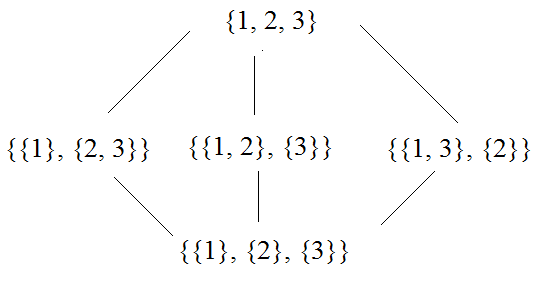
\includegraphics[width=0.5\linewidth]{hasse}
\centering
\end{figure}

\end{document}